\documentclass[11pt]{article}
\usepackage[margin=1in]{geometry}
\usepackage{graphicx}
\usepackage{booktabs}
\usepackage{amsmath}
\usepackage[hidelinks]{hyperref}
\usepackage{url}

\title{Direct Current Subtransmission Backbone for AI Factories:\\
A Position Paper with Source-Anchored Architecture Modeling and OpenDSS Boundary Cross-Checks}

\author{Author Name(s) Here}
\date{April 2026}

\begin{document}
\maketitle

\begin{abstract}
AI factories are becoming power-delivery-limited before they become compute-limited. The conventional response has been to improve the last portion of the power path, especially by introducing higher-voltage facility buses such as 800~VDC. That direction is necessary, but it is incomplete if alternating current still penetrates the campus deeply enough to recreate repeated conversion, distributed power-quality ownership, and reactive-power coordination across multiple pods or facility front ends. This paper takes the position that the next architectural step is to move the main AC/DC boundary upstream to the campus subtransmission interface and to treat the downstream campus as a DC-native system.

To support that position, this paper combines a source-anchored comparative architecture model with OpenDSS quasi-static AC-boundary cross-checks, a standardized harmonic-sensitivity scan, and a follow-on multi-node campus comparison. Three base scenarios are compared at a 100~MW delivered IT reference campus: Scenario~1, a traditional AC-centric path; Scenario~2, an NVIDIA-style 69~kV AC to 800~VDC perimeter-conversion path; and Scenario~3, a proposed 69~kV-class medium-voltage direct-current (MVDC) backbone feeding isolated DC pods and an 800~VDC facility bus. A second model layer then compares Scenario~1(M), Scenario~2(M), and Scenario~3(M) on the same four-block campus topology. In the corrected present model, the MVDC backbone remains directionally favorable in both the single-path and multi-node comparisons, while the OpenDSS layers indicate lower modeled AC-side feeder burden and lower AC-boundary harmonic sensitivity when the AC/DC boundary is centralized. The dynamic-load analysis further shows that AI-factory power architecture should be evaluated under time-varying load envelopes, not only steady-state energy accounting.

The paper does not claim that the present model closes all deployment questions. Protection, grounding, harmonic compliance, converter-control dynamics, and proxy-parameter uncertainty still require deeper study. The position advanced here is therefore directional rather than final: once AI factories are recognized as large, converter-rich, dynamic loads, a DC subtransmission backbone becomes a credible system architecture that merits deeper validation.
\end{abstract}

\section{Introduction}
AI data centers are entering a regime in which electrical infrastructure increasingly determines scalability. Public demand forecasts already place data centers among the fastest-growing large loads on the grid, while recent AI-factory designs concentrate that demand into highly power-dense campuses \cite{IEA2025EnergyAI,LBL2025DataCenterDemand,NVIDIA2025SuperPOD}. At the same time, public and utility-facing studies now show that AI-training facilities behave as dynamic electrical loads rather than purely static loads \cite{PNNL2026EMT,Choukse2025PowerStabilization,Mishra2025Oscillation}. These shifts mean that power architecture can no longer be framed as a rack-level efficiency detail alone.

The conventional campus path remains largely AC-centric. Power enters through AC subtransmission, continues through AC primary distribution, and then encounters a cascade of transformation and conversion stages before it reaches the GPU voltage-regulation stages. Even when modern facility designs adopt 800~VDC internally, AC often remains present up to the facility or pod boundary \cite{NVIDIA2025HVDCBlog}. That approach improves the last segment of the power path, but it leaves the campus-level architecture partially unresolved.

This paper advances a position: the correct next move is to establish a DC subtransmission backbone. In that architecture, a common subtransmission AC/DC front end is placed at the campus entry. Downstream of that point, the campus backbone is DC-native, isolation is provided by isolated DC pods or DC transformers, and the facility side remains consistent with the emerging 800~VDC direction. The argument is not that every implementation detail has been solved. The argument is that this architecture is the right reference point for solving the remaining details.

\section{Position}
The central claim is that AI-factory power architecture should stop at neither the low-voltage bus nor the pod front end. If the load is increasingly DC-native and the dominant controllable resources such as batteries and photovoltaics are also DC-native, then extending AC deeply into the campus creates avoidable architectural friction.

This position rests on four propositions.

First, repeated high-power conversion stages create a multiplicative efficiency penalty. Optimizing only one stage cannot recover the architectural losses introduced by keeping several large stages in series \cite{Pratt2007DC,Shrestha2018ACDC,Rothmund2019DCXfmr}.

Second, AI factories are dynamic loads. Public studies now describe periodic and grid-relevant power fluctuations in large AI-training sites, while utility measurements show that data-center-rich regions can exhibit nontrivial oscillatory behavior linked to power-electronic loads \cite{PNNL2026EMT,Choukse2025PowerStabilization,Mishra2025Oscillation}. A campus architecture must therefore be judged by its dynamic interaction with the grid as well as by its steady-state efficiency.

Third, power-quality ownership becomes easier to define when the AC side is centralized. If the campus has one common AC/DC front end, then harmonics and power-factor behavior are concentrated at the grid interface rather than recreated at many downstream AC front ends.

Fourth, a DC backbone is a more natural integration domain for batteries, photovoltaics, and local energy buffers. That does not eliminate the need for sophisticated controls, but it removes unnecessary AC/DC/AC detours from the resource path.

\section{Scenarios Under Comparison}
This paper compares three scenarios derived from the supporting model files in the project workspace.

\begin{figure}[t]
    \centering
    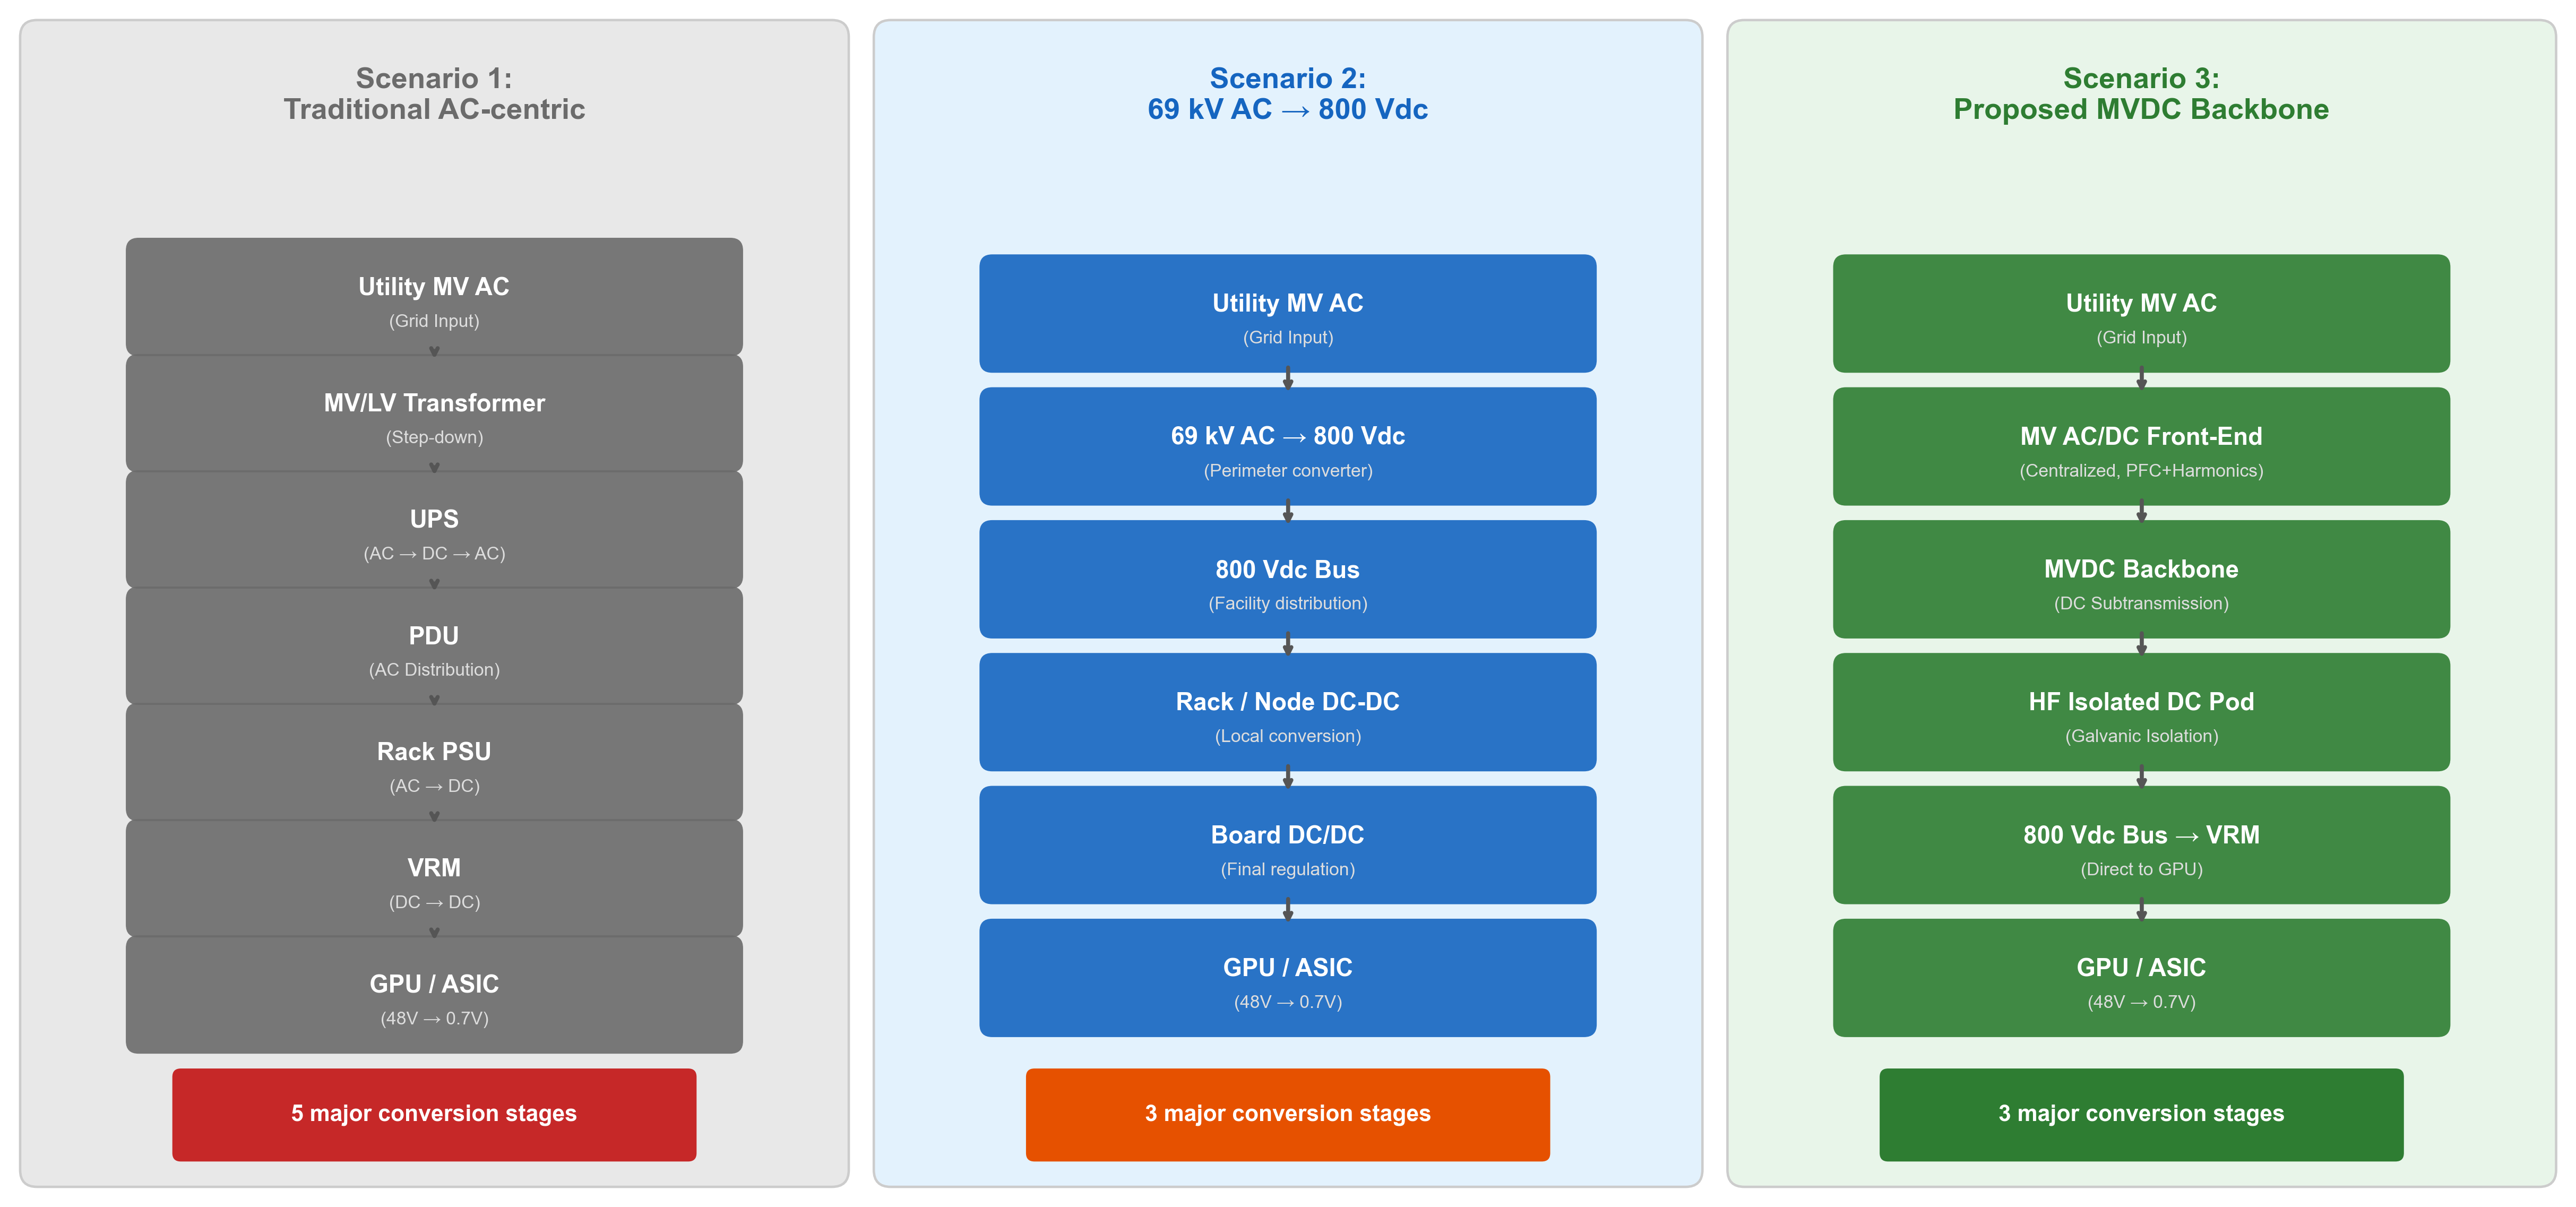
\includegraphics[width=\linewidth]{figures/architecture_comparison.png}
    \caption{Three scenarios used throughout this paper. Scenario~3 moves the main AC/DC boundary upstream and keeps the campus DC-native downstream of the centralized front end.}
    \label{fig:architecture}
\end{figure}

\subsection{Scenario 1: Traditional AC-centric baseline}
The baseline keeps AC as the dominant campus-distribution domain. The representative path is a 69~kV AC campus feeder, medium-voltage to low-voltage transformation, facility UPS, low-voltage AC distribution, a PDU or transformer stage, server AC/DC conversion, and board-level DC/DC regulation.

\subsection{Scenario 2: NVIDIA-style 69~kV AC to 800~VDC perimeter conversion}
Scenario~2 is intended to reflect the direction of an 800~VDC facility while preserving AC upstream of the facility boundary. In the current scenario, a 69~kV AC campus feeder supplies a direct 69~kV AC to 800~VDC perimeter-conversion stage, followed by an 800~VDC facility bus, rack or node DC/DC conversion, and board-level DC/DC conversion. The 800~VDC downstream structure is source-backed; the 69~kV campus-side voltage is a local scenario assumption requested for this study \cite{NVIDIA2025HVDCBlog}. Scenario~2 is therefore an important advanced comparator, but it still stops short of an MVDC backbone.

\subsection{Scenario 3: Proposed MVDC backbone}
Scenario~3 centralizes the AC/DC boundary at the campus entry. A centralized 69~kV-class AC/DC front end feeds an MVDC backbone, which then supplies isolated DC pods or DC transformers, the 800~VDC facility bus, rack or node DC/DC conversion, and board-level DC/DC regulation. This is the main architectural contribution of the paper. The key system-level change is not merely the use of better converters; it is the relocation of the main AC/DC boundary and the explicit introduction of the MVDC backbone as the campus organizing layer while preserving the same end-use electrical boundary as Scenario~2.

\section{Modeling Framework}
\subsection{Source-anchored architecture model}
The first model layer is an architecture comparison model implemented in Python. It evaluates each path from the delivered IT load back to the upstream source by traversing a sequence of stages and conductors. The path efficiency is computed by combining stage efficiencies with conductor losses:
\begin{equation}
\eta_{\text{path}} = \frac{P_{\text{IT}}}{P_{\text{source}}}.
\end{equation}
Partial-load converter efficiencies are represented with source-anchored or explicitly labeled proxy curves. The present assumptions are stored in a source-tagged JSON file so that each major input can be traced to a public source, a local scenario assumption, or a documented proxy.

\subsection{Dynamic-load layer}
The analytical model also includes dynamic AI-load cases. Two frequency anchors are used. The first is a 1.0~Hz reference point within the 0.1--5~Hz band that PNNL identifies as relevant for positive-sequence dynamic studies \cite{PNNL2026EMT}. The second is a measured 14.8~Hz case drawn from a real data-center oscillation study in Dominion Energy territory \cite{Mishra2025Oscillation}. Amplitude values are sensitivity cases rather than universal measured constants. For each case, the model estimates the raw PCC power swing and the native buffer power and energy that would be required at the architecture's natural support point.

\subsection{OpenDSS cross-check layer}
The second model layer uses OpenDSS as an AC-side quasi-static cross-check tool \cite{OpenDSS2026}. This layer is intentionally narrow. It does not attempt to model the internal MVDC backbone or the 800~VDC plant in electromagnetic-transient detail. Instead, it models the upstream AC source, the AC feeder or substation-side AC stub, and the equivalent downstream demand seen at that AC boundary.

For Scenarios~1 and~2, the first modeled 69~kV AC feeder is preserved in OpenDSS. For Scenario~3, the long AC feeder inside the campus is replaced by a short centralized-front-end AC stub because the AC/DC conversion is assumed to occur at the campus entry. This is a surrogate representation of the scenario boundary shift, not a claim of an already-standardized utility model.

The OpenDSS study is executed as a sequence of quasi-static snapshots over two cycles with 64 samples per cycle. At each time step, the downstream demand is updated from the analytical model and the resulting source power, feeder current, feeder loss, and PCC voltage are recorded.

\subsection{Multi-node campus extension}
The single-path architecture comparison is useful for isolating end-to-end conversion structure, but it is not by itself a campus-topology model. To address that limitation, a separate multi-node comparison is also run on a shared four-block campus layout. In that extension, Scenario~1(M), Scenario~2(M), and Scenario~3(M) use the same block sizes, tap locations, and inter-block segment lengths. Scenario~1(M) and Scenario~2(M) retain a 69~kV AC backbone, while Scenario~3(M) replaces that campus-interior AC backbone with a 69~kV DC backbone. Each block then carries its scenario-specific local conversion path to the IT load.

This extension is intentionally still simplified: it is radial, balanced, and quasi-static, and it does not yet represent protection, N--1 reconfiguration, or converter-control transients. Its role is narrower. It checks whether the ranking observed in the simpler single-path model survives when the scenarios are forced onto the same explicit multi-block campus topology.

\subsection{Source basis and limitations}
The strongest public anchors in this study come from the IEA, EIA, PNNL, official NVIDIA materials, Open Compute Project data, Schneider Electric specifications, and peer-reviewed literature on DC power conversion and data-center dynamics \cite{IEA2025EnergyAI,EIA2026Monthly,NVIDIA2025SuperPOD,NVIDIA2025HVDCBlog,PNNL2026EMT,OCP2026Delta,Schneider2025GalaxyVX,Rothmund2019DCXfmr,Mishra2025Oscillation}. Some key quantities remain proxy-based, especially the exact partial-load curves for the centralized medium-voltage rectifier and the isolated DC pod stage. Those proxies are labeled accordingly in the model artifacts, and the resulting ranking should be interpreted as conditional on those assumptions rather than as a finalized deployment result.

\section{Results}
\subsection{Steady-state architecture results}
Figure~\ref{fig:efficiency} shows the cumulative-efficiency thesis graphically, while Table~\ref{tab:steady} gives the current quantitative results for the 100~MW reference campus.

\begin{figure}[t]
    \centering
    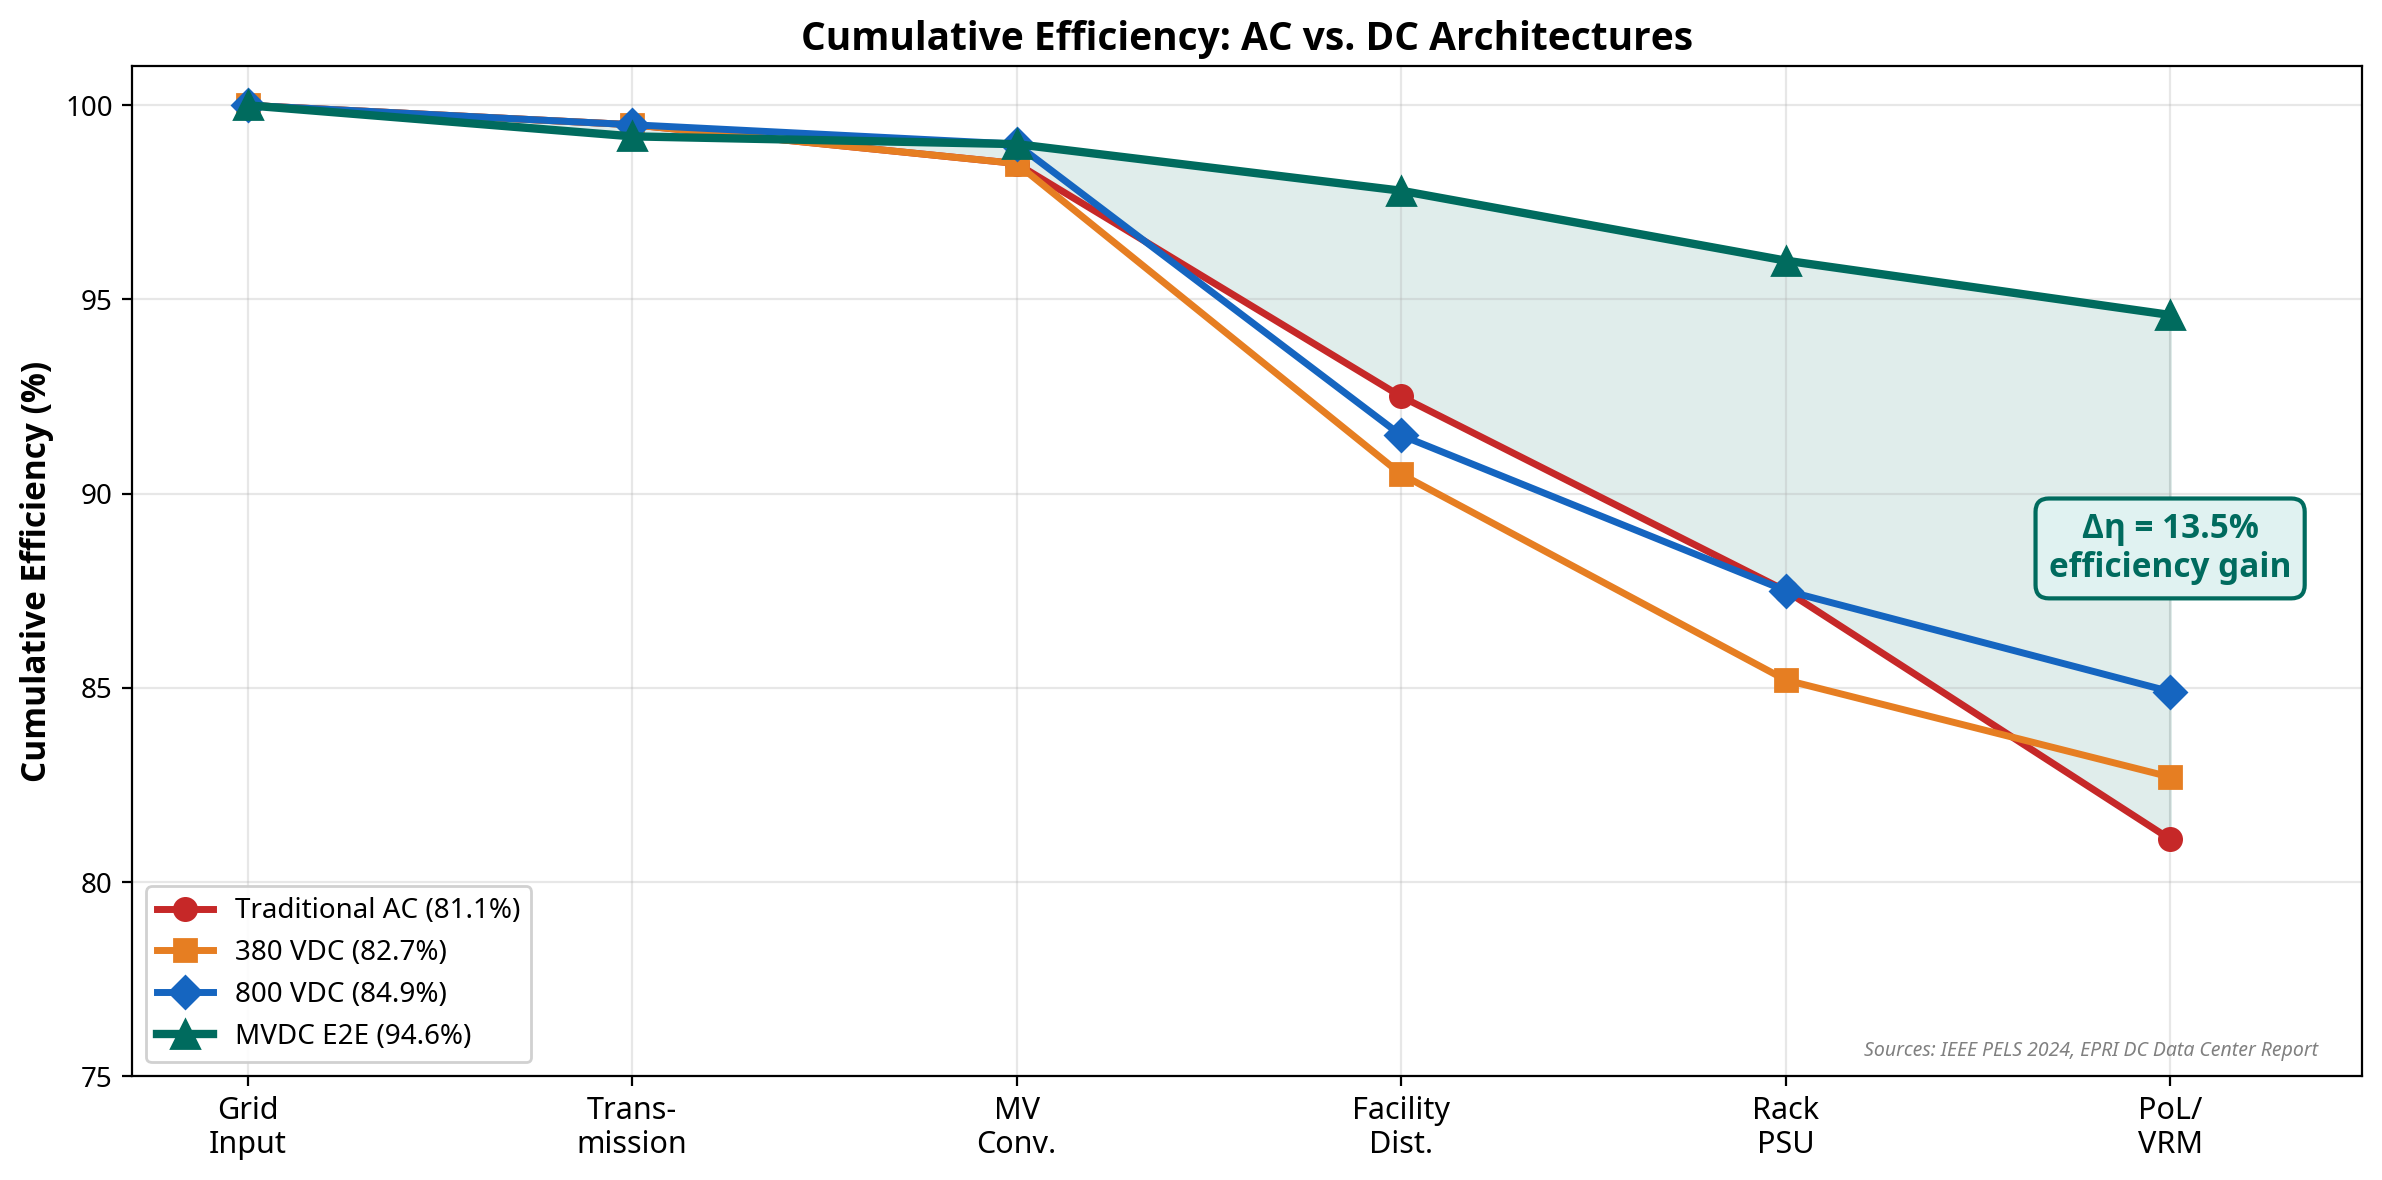
\includegraphics[width=\linewidth]{figures/cumulative_efficiency.png}
    \caption{Cumulative-efficiency comparison for the three evaluated scenarios. The values shown are taken from the current source-anchored model outputs.}
    \label{fig:efficiency}
\end{figure}

\begin{table}[t]
    \centering
    \caption{Steady-state comparison at 100~MW delivered IT load}
    \label{tab:steady}
    \begin{tabular}{p{2.5in}cccc}
        \toprule
        Scenario & Full-load eff. & Input MW & Loss GWh/yr & Loss cost (\$M/yr) \\
        \midrule
        Scenario~1: Traditional AC-centric & 87.48\% & 114.31 & 125.36 & 11.65 \\
        Scenario~2: 69~kV AC to 800~VDC perimeter conversion & 91.90\% & 108.81 & 77.21 & 7.17 \\
        Scenario~3: Proposed MVDC backbone & 92.17\% & 108.50 & 74.45 & 6.92 \\
        \bottomrule
    \end{tabular}
\end{table}

The steady-state result is materially traceable and still architecturally relevant after correcting the scenario endpoint. Scenario~3 remains the numerically best case, but the margin over Scenario~2 is modest: about 0.27 percentage points in full-load efficiency and about 2.76~GWh in annualized losses under the reference continuous-operation profile. That smaller margin matters. It means the strongest remaining argument for Scenario~3 is no longer a dramatic single-path efficiency gain alone, but a combination of directional efficiency benefit, centralized AC interaction, and a cleaner campus-scale DC architecture.

\subsection{Dynamic-load results}
The need for a dynamic model is motivated by the public evidence that AI-training facilities can exhibit periodic power swings and grid-relevant interactions. Figure~\ref{fig:gpu} summarizes the dynamic-load motivation, and Table~\ref{tab:dynamic} presents selected dynamic results from the analytical model.

\begin{figure}[t]
    \centering
    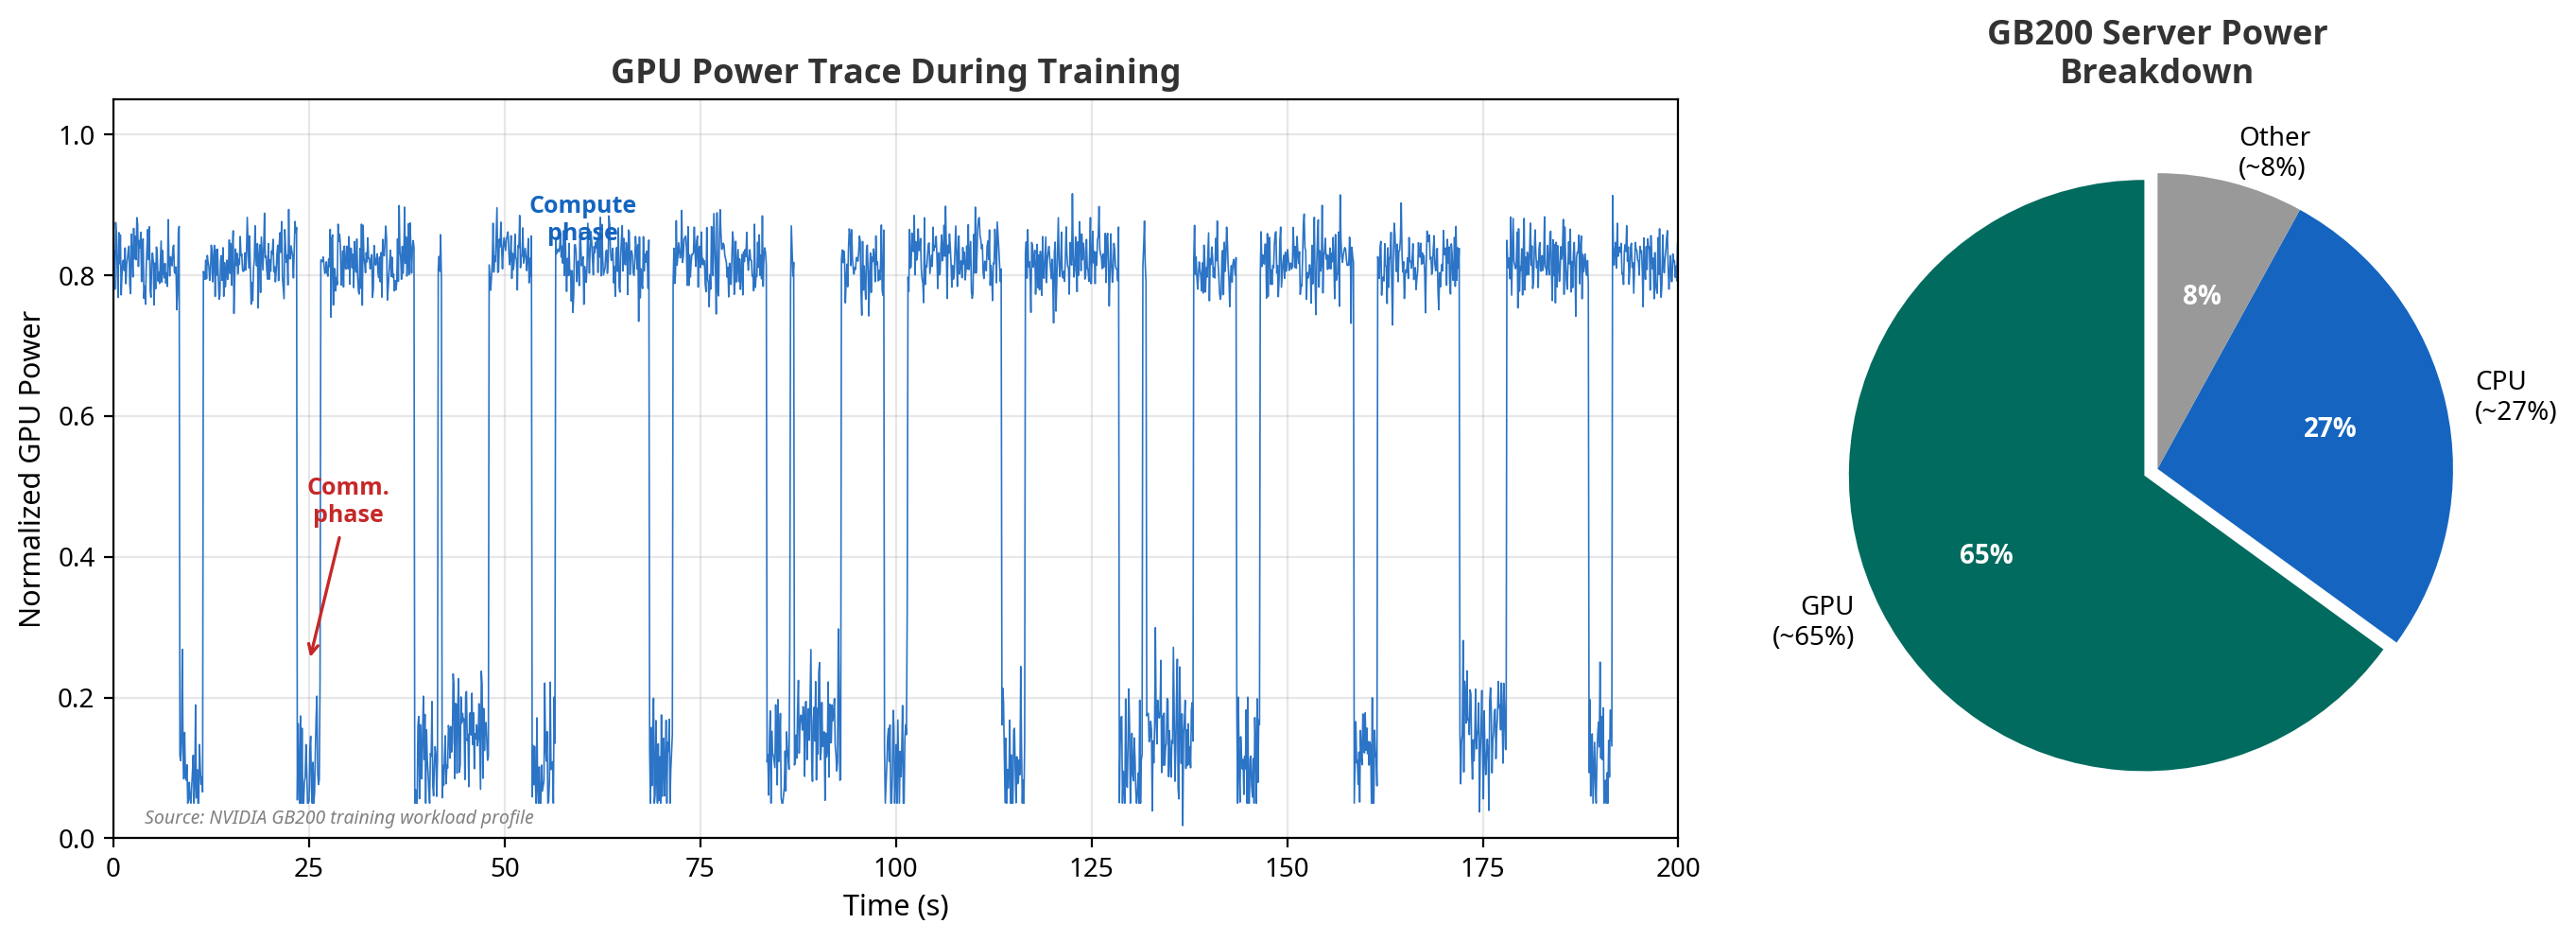
\includegraphics[width=\linewidth]{figures/gpu_power_trace.png}
    \caption{Motivation figure emphasizing the dynamic power profile of AI training and the dominance of GPU power in advanced AI systems.}
    \label{fig:gpu}
\end{figure}

\begin{table}[t]
    \centering
    \caption{Selected analytical dynamic-load results}
    \label{tab:dynamic}
    \begin{tabular}{p{1.55in}p{1.15in}ccc}
        \toprule
        Scenario & Case & Raw PCC peak (MW) & Native buffer (MW) & Native buffer (kWh) \\
        \midrule
        Scenario~1: Traditional AC-centric & 1.0~Hz, 15\% IT amplitude & 17.09 & 15.20 & 0.67 \\
        Scenario~2: 69~kV AC to 800~VDC perimeter conversion & 1.0~Hz, 15\% IT amplitude & 16.31 & 15.40 & 0.68 \\
        Scenario~3: Proposed MVDC backbone & 1.0~Hz, 15\% IT amplitude & 16.26 & 15.47 & 0.68 \\
        \midrule
        Scenario~1: Traditional AC-centric & 14.8~Hz, 10\% IT amplitude & 11.35 & 10.14 & 0.03 \\
        Scenario~2: 69~kV AC to 800~VDC perimeter conversion & 14.8~Hz, 10\% IT amplitude & 10.83 & 10.27 & 0.03 \\
        Scenario~3: Proposed MVDC backbone & 14.8~Hz, 10\% IT amplitude & 10.80 & 10.31 & 0.03 \\
        \bottomrule
    \end{tabular}
\end{table}

Two points are important. First, the scenario ranking remains slightly favorable to Scenario~3 when the load is treated dynamically rather than only statically. Second, the margin between scenarios is smaller in the dynamic power-swing metric than in the annual energy metric, which is exactly why dynamic modeling is required. A paper that only reported annual losses would miss an essential part of the AI-factory problem. The correct interpretation is therefore not that Scenario~3 is decisively proven by this layer; it is that the MVDC backbone remains directionally favorable even after the comparison is widened beyond steady-state efficiency.

\subsection{OpenDSS AC-boundary cross-check}
The OpenDSS results add a feeder-side cross-check perspective. Table~\ref{tab:opendssbase} reports the 100~MW base-case AC-boundary results, and Table~\ref{tab:opendssstress} reports selected dynamic stress results.

\begin{table}[t]
    \centering
    \caption{OpenDSS base-case AC-boundary cross-check}
    \label{tab:opendssbase}
    \begin{tabular}{p{2.25in}cccc}
        \toprule
        Scenario & Source MW & PCC min pu & Feeder loss (MW) & Peak current (A) \\
        \midrule
        Scenario~1: Traditional AC-centric & 114.48 & 0.9707 & 0.194 & 1005 \\
        Scenario~2: 69~kV AC to 800~VDC perimeter conversion & 108.95 & 0.9722 & 0.175 & 955 \\
        Scenario~3: Proposed MVDC backbone & 108.49 & 0.9742 & 0.004 & 951 \\
        \bottomrule
    \end{tabular}
\end{table}

\begin{table}[t]
    \centering
    \caption{OpenDSS dynamic stress results at the AC boundary}
    \label{tab:opendssstress}
    \begin{tabular}{p{1.55in}p{1.05in}ccc}
        \toprule
        Scenario & Case & Source peak (MW) & Max PCC swing & Peak feeder loss (MW) \\
        \midrule
        Scenario~1: Traditional AC-centric & 1.0~Hz, 15\% IT amplitude & 17.15 & 0.50\% & 0.259 \\
        Scenario~2: 69~kV AC to 800~VDC perimeter conversion & 1.0~Hz, 15\% IT amplitude & 16.38 & 0.47\% & 0.234 \\
        Scenario~3: Proposed MVDC backbone & 1.0~Hz, 15\% IT amplitude & 16.27 & 0.44\% & 0.006 \\
        \midrule
        Scenario~1: Traditional AC-centric & 14.8~Hz, 10\% IT amplitude & 11.39 & 0.33\% & 0.236 \\
        Scenario~2: 69~kV AC to 800~VDC perimeter conversion & 14.8~Hz, 10\% IT amplitude & 10.89 & 0.31\% & 0.213 \\
        Scenario~3: Proposed MVDC backbone & 14.8~Hz, 10\% IT amplitude & 10.82 & 0.29\% & 0.005 \\
        \bottomrule
    \end{tabular}
\end{table}

These results should be interpreted as cross-checks of the upstream AC-boundary consequences of the scenario definitions, not as independent site-specific validation. The comparison model alone shows that Scenario~3 has the lowest end-to-end loss. The OpenDSS layer adds that the same scenario also yields the lightest modeled AC-side burden at the campus boundary. In the present scenario, the AC-boundary feeder loss in Scenario~3 is approximately two orders of magnitude lower than in Scenarios~1 and~2 because the long campus-interior AC feeder is removed from the scenario definition. That does not prove a utility interconnection result. It does show that the backbone architecture has a direct and favorable implication at the modeled AC boundary.

\subsection{OpenDSS harmonic-sensitivity scan}
The present paper also adds a standardized OpenDSS harmonic-sensitivity scan at the AC boundary. This is not an IEEE~519 compliance study. Instead, the same three-phase harmonic current probe is injected at the PCC for each scenario at the 5th, 7th, 11th, and 13th harmonic orders, and the resulting harmonic voltage distortion is compared across scenarios. The point of the scan is to test whether the centralized-front-end architecture creates a less sensitive AC boundary under the same perturbation basis.

\begin{table}[t]
    \centering
    \caption{OpenDSS harmonic-sensitivity scan at the AC boundary}
    \label{tab:harmonicprobe}
    \begin{tabular}{p{2.25in}ccc}
        \toprule
        Scenario & Probe THD$_v$ (\%) & Max transfer impedance ($\Omega$, L--N) & Interpretation \\
        \midrule
        Scenario~1: Traditional AC-centric & 10.02 & 215.05 & Most sensitive AC boundary \\
        Scenario~2: 69~kV AC to 800~VDC perimeter conversion & 9.57 & 205.54 & Reduced sensitivity versus Scenario~1 \\
        Scenario~3: Proposed MVDC backbone & 9.30 & 199.91 & Lowest sensitivity in the present scan \\
        \bottomrule
    \end{tabular}
\end{table}

The harmonic-sensitivity result does not establish formal compliance margins, but it does add quantitative support to the power-quality argument. The architecture with the most centralized AC interface also produces the lowest voltage-distortion response under the same harmonic-current probe. That is a stronger basis for the power-quality claim than topology alone.

\subsection{Multi-node campus comparison}
Table~\ref{tab:multinode} reports the follow-on campus comparison in which all three scenarios are mapped onto the same four-block topology. This is the strongest topology-level check in the present paper because it removes the objection that Scenario~3 only wins in an overly collapsed equivalent path.

\begin{table}[t]
    \centering
    \caption{Shared-campus multi-node comparison at 100~MW total IT load}
    \label{tab:multinode}
    \begin{tabular}{p{2.1in}cccc}
        \toprule
        Scenario & Full-load eff. & Source MW & Loss GWh/yr & Worst dynamic source peak (MW) \\
        \midrule
        Scenario~1(M): Traditional AC-centric & 81.11\% & 123.29 & 204.05 & 17.86 \\
        Scenario~2(M): 69~kV AC to 800~VDC perimeter conversion & 86.19\% & 116.03 & 140.38 & 16.92 \\
        Scenario~3(M): Multi-node MVDC backbone & 86.69\% & 115.36 & 134.55 & 16.81 \\
        \bottomrule
    \end{tabular}
\end{table}

The shared-campus result is important for two reasons. First, the ranking remains unchanged: the MVDC-backbone case still performs best when the campus is represented as multiple data-center blocks rather than one equivalent path. Second, the gap between Scenario~3(M) and Scenario~2(M) is again modest rather than dramatic, which means the multi-node model supports the architecture direction but does not, by itself, close the case. That is exactly the right interpretation for a position paper rather than a deployment paper.

\subsection{Proxy-robustness stress test}
Because several advanced-converter curves remain proxy-based, the paper also includes a simple robustness check on the three most consequential proxy curves: the 69~kV AC to 800~VDC perimeter converter, the centralized MV AC/DC front end, and the isolated DC pod stage. In that stress test, each of the three curves is shifted by $\pm$1 percentage point in additive efficiency offset over a five-point grid, yielding 125 combined cases.

The stress test shows that the ranking is not fully robust to proxy uncertainty. Scenario~3 remains more efficient than Scenario~2 in 69 of the 125 single-path cases, and Scenario~3(M) remains more efficient than Scenario~2(M) in 88 of the 125 multi-node cases. This is a useful result precisely because it is not uniformly favorable: it shows that measured front-end and isolated-pod efficiency data are not a cosmetic refinement but a gating requirement for a journal-grade quantitative claim.

\section{Discussion}
The results support three main conclusions: lower end-to-end loss, cleaner power-quality ownership, and simpler integration of DC-native resources. The evidence for each conclusion has a different strength, and that distinction matters.

The loss-reduction conclusion is supported most directly, but it is also the conclusion most constrained by proxy uncertainty. The steady-state model shows a clear ranking across Scenario~1, Scenario~2, and Scenario~3, and that ranking remains meaningful even when Scenario~2 is included as a strong advanced comparator rather than only the traditional baseline. More importantly, the ranking survives the multi-node extension in Table~\ref{tab:multinode}. At the same time, the proxy-robustness stress test shows that the margin between Scenario~2 and Scenario~3 is not insensitive to front-end and isolated-pod assumptions. The current evidence therefore supports a directional efficiency preference, not a large or fully settled quantitative advantage.

The power-quality conclusion is now supported more directly, although still not at full compliance-study strength. The architecture comparison reduces the number of AC-side interaction points from four in the traditional case to one in the two advanced cases. The added OpenDSS harmonic-sensitivity scan also shows the lowest probe THD$_v$ and the lowest transfer impedance in Scenario~3 under the same injected harmonic-current basis. This still does not replace a full IEEE~519 study with converter-specific spectra and utility short-circuit data. It does, however, move the paper beyond a purely topological power-quality argument.

The DC-native-integration conclusion is also supported directionally. The dynamic model's native-buffer calculations show that the natural support point of the MVDC architecture sits inside the DC domain rather than behind repeated AC boundaries. That does not yet quantify the best battery placement or control law. It does show that the architecture aligns the buffering problem with the same electrical domain as the load.

The present model is strong enough to defend three statements:
\begin{itemize}
    \item Moving from Scenario~2 to Scenario~3, not only from Scenario~1 to Scenario~3, improves end-to-end electrical-path efficiency in the corrected present source-anchored scenario, although the margin is modest.
    \item That same ranking survives the added four-block campus comparison across Scenario~1(M), Scenario~2(M), and Scenario~3(M).
    \item AI-factory architecture should be evaluated under dynamic-load conditions, not only annual energy accounting.
    \item An AC-boundary OpenDSS cross-check shows lower feeder current, lower feeder loss, lower PCC voltage swing, and lower harmonic-sensitivity response when the campus-interior AC path is removed.
\end{itemize}

The paper should not yet claim that the present model proves exact harmonic compliance, exact converter-control stability margins, or deployable MVDC protection settings. Those are the right next topics, but they are not required for a strong position paper.

\section{Research Priorities}
The present results establish a defensible architecture-level case for an MVDC backbone, but several research questions remain open before the concept can be treated as deployment-ready. The most important next steps are the following.

\begin{itemize}
    \item \textbf{Protection and grounding:} Develop equipment-specific fault-clearing, grounding, insulation-coordination, and sectionalization concepts for the MVDC backbone.
    \item \textbf{Converter characterization:} Replace proxy efficiency curves with vendor-qualified or experimentally measured curves for the centralized rectifier and isolated DC pod stages.
    \item \textbf{PCC studies:} Extend the present AC-boundary model into a site-specific interconnection study using utility Thevenin equivalents, harmonic limits, and short-circuit data.
    \item \textbf{Dynamic controls:} Move from the present quasi-static and analytical dynamic layers to converter-aware EMT studies with explicit control models for the centralized front end, isolated DC pod, and supporting buffers.
    \item \textbf{Buffer placement:} Determine the preferred placement and control role of subsecond energy buffers across the GPU, rack, pod, and backbone levels.
\end{itemize}

Among these topics, the highest-value next modeling step is an EMT-grade validation of the centralized front end, isolated DC pod, and buffer controls under weak-grid and disturbance scenarios. That step would materially strengthen the case that the architecture remains favorable not only in steady-state comparisons, but also under converter-driven transient conditions that matter for large AI-factory interconnections.

\section{Conclusion}
This paper argues that the next logical move after the 800~VDC facility bus is to seriously evaluate a DC subtransmission backbone. The position is motivated by three facts that now occur together: AI factories are becoming very large loads, they are increasingly dynamic loads, and the dominant controllable resources around them are already DC-native.

The current source-anchored model supports that position directionally rather than conclusively. At the 100~MW reference campus, Scenario~3, the proposed MVDC backbone, achieves the best full-load efficiency and the lowest annualized reference-profile losses among the three evaluated scenarios, but its margin over Scenario~2 is modest. The dynamic-load layer further shows that the architecture question does not disappear when AI loads are treated as time-varying. The OpenDSS cross-check adds a second result: pushing the AC boundary upstream reduces the modeled AC-side feeder burden at the campus boundary.

The follow-on multi-node comparison strengthens that conclusion further, but it also disciplines it. When all three scenarios are forced onto the same explicit four-block campus topology, the MVDC-backbone case still yields the best efficiency, the lowest annualized reference-profile loss, and the smallest worst-case source swing in the present dynamic stress set. The result is therefore not confined to a one-line equivalent architecture model, but it is also not yet strong enough to eliminate the need for measured converter data and EMT-grade validation.

The result is not a claim that every deployment question is finished. It is a claim that the right reference architecture has become visible. For AI factories, the higher-value move is no longer only a better facility front end. It is a campus architecture that treats the DC nature of the load as a first-order design principle.

\section*{Reproducibility Note}
The quantitative results in this manuscript are generated from the project files \texttt{dc\_backbone\_model.py}, \texttt{scientific\_assumptions\_v1.json}, \texttt{source\_backed\_model\_report.json}, \texttt{dc\_backbone\_multinode\_campus\_model.py}, and \texttt{multinode\_campus\_report.json}. The single-path OpenDSS validation can be reproduced with:
\begin{verbatim}
python3 dc_backbone_model.py --run-opendss \
  --save-json source_backed_model_report.json \
  --write-memo MODEL_RESULTS_MEMO.md
\end{verbatim}
The multi-node campus comparison can be reproduced with:
\begin{verbatim}
python3 dc_backbone_multinode_campus_model.py \
  --save-json multinode_campus_report.json
\end{verbatim}

\bibliographystyle{IEEEtran}
\bibliography{references}

\end{document}
